	% !TEX TS-program = xelatex
\documentclass[12pt, reqno]{amsart}
\usepackage{amsmath, amsthm, amscd, amsfonts, amssymb, graphicx, color}
\usepackage[margin=2.5cm]{geometry}

\usepackage{tikz}
\usetikzlibrary{lindenmayersystems, shadings, backgrounds}
\definecolor{dragonRed}{RGB}{200, 40, 40}
\definecolor{dragonBlue}{RGB}{40, 80, 200}

\pgfdeclarelindenmayersystem{Dragon}{
    \symbol{X}{\pgflsystemdrawforward}
    \symbol{Y}{\pgflsystemdrawforward}
    \rule{X -> X+YF+}
    \rule{Y -> -FX-Y}
}

\usepackage{xepersian}

\settextfont[Path=./, Extension=.ttf, Scale=1.2]{XB Niloofar}
\setlatintextfont[Scale=1.0]{Latin Modern Roman}
\setdigitfont[Path=./, Extension=.ttf, Scale=1.1]{XB Zar}

\def\affilfont{\normalfont\fontsize{11}{13}\selectfont\centering}
\def\affil#1{\par\vskip12pt{\affilfont#1\par}\vskip15pt}
\def\authorsaddresses#1{\dedicatory{\vskip 0.5em \small #1}}

\newtheorem{theorem}{قضیه}[section]
\newtheorem{definition}[theorem]{تعریف}
\numberwithin{equation}{section}

\begin{document}
\setcounter{page}{1}

\title[منحنی اژدهای دیویس-کنوث] 
{ساختار هندسی، نمایش اعداد و پیاده‌سازی\\ منحنی اژدهای دیویس-کنوث}

\author[علیرضا زارع بیدکی]{علیرضا زارع بیدکی}

\authorsaddresses{
    دانشکده علوم ریاضی، دانشگاه فردوسی مشهد \\
    \lr{\tt alireza.zarebidoki@mail.um.ac.ir}
}

\begin{abstract}
منحنی اژدها که با نام‌های «اژدهای هایوی» یا «فراکتال کاغذ تاشده» نیز شناخته می‌شود، ساختاری خودهمانند است که نخستین بار توسط فیزیکدانان ناسا کشف شد. اما اهمیت اصلی آن در علوم کامپیوتر، مدیون مقاله جریان‌ساز دیویس و کنوث (۱۹۷۰) است که ارتباط این منحنی را با نمایش اعداد در مبناهای مختلط آشکار ساختند. در این مقاله، ضمن پیاده‌سازی الگوریتم رسم با استفاده از سامانه «ال-سیستم» و بسته «تیکز»، به بررسی ویژگی «فرش‌کردن صفحه» و کاربردهای نوین آن در مقالات سال ۲۰۲۵ می‌پردازیم.

\bigskip
\noindent \textbf{کلید واژگان:} منحنی اژدها، سیستم لیندن‌مایر، اعداد مختلط، فرش‌کردن صفحه، فراکتال.
\end{abstract}

\maketitle

\section{مقدمه: از کاغذ تا اعداد مختلط}
اگر نوار کاغذی را $n$ بار به صورت متوالی از وسط تا کنیم و سپس آن را با زوایای ۹۰ درجه باز کنیم، منحنی اژدها\footnote{\lr{Dragon Curve}} پدیدار می‌شود. اما آنچه این منحنی را از نظر ریاضیاتی برجسته می‌کند، ارتباط آن با سیستم اعداد باینری در صفحه مختلط است.
پروفسور دونالد کنوث و چندلر دیویس در مقاله مشهور خود \cite{davis1970} نشان دادند که این منحنی فراتر از یک بازی با کاغذ است. به بیان دقیق‌تر، همانطور که هر عدد صحیح را می‌توان در مبنای ۲ نوشت، هر عدد صحیح مختلط\footnote{\lr{Gaussian Integer}} را می‌توان به صورت یکتا در مبنای $b = -1+i$ با ارقام $\{0, 1\}$ نمایش داد.

\section{ویژگی‌های هندسی و الگوریتم رسم}\label{sec2}
برای رسم این منحنی در کامپیوتر، از سیستم‌های لیندن‌مایر\footnote{\lr{L-System}} استفاده می‌شود. این سیستم یک روش بازنویسی رشته‌ای موازی است.

\subsection{الگوریتم تولید}
قواعد تولید این فراکتال به صورت زیر تعریف می‌شود:
\[
    X \rightarrow X+YF+, \quad Y \rightarrow -FX-Y
\]
که در آن $F$ گام به جلو، $+$ چرخش ۹۰ درجه راست‌گرد و $-$ چرخش ۹۰ درجه چپ‌گرد است.

\section{پیاده‌سازی و شبیه‌سازی در \lr{\LaTeX}}

\subsection{رسم منحنی تک‌رشته‌ای}
در شکل \ref{fig:single_dragon}، منحنی اژدها تا مرحله ۱۱ با استفاده از بسته تیکز\footnote{\lr{TikZ}} ترسیم شده است. این تکنیک بصری ثابت می‌کند که منحنی هرگز خود را قطع نمی‌کند، بلکه صرفاً رئوس خود را لمس می‌کند.

\begin{figure}[ht]
    \centering
    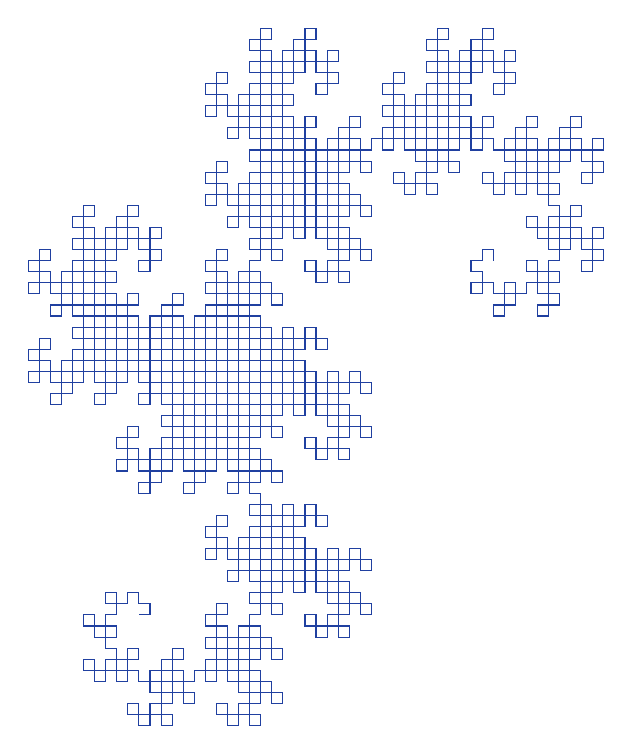
\begin{tikzpicture}
        \draw [draw=dragonBlue!80!black, line width=0.4pt, rotate=90]
        [l-system={Dragon, step=2pt, axiom=FX, order=11, angle=90}]
        lindenmayer system;
    \end{tikzpicture}
    \caption{منحنی اژدهای مرتبه ۱۱. تراکم خطوط در مرکز نشان‌دهنده ماهیت فضاپُرکن این منحنی است.}
    \label{fig:single_dragon}
\end{figure}

\subsection{اژدهای دوقلو و خاصیت فرش‌کردن}
یکی از زیباترین خواص این فراکتال که در مقاله نوین سال ۲۰۲۵ نیز مورد بحث قرار گرفته است \cite{arxiv2025}، قابلیت آن در پوشاندن کامل صفحه است (خاصیت \lr{Tiling}). اگر دو منحنی اژدها را (یکی با چرخش ۱۸۰ درجه نسبت به دیگری) رسم کنیم، مانند قطعات پازل در هم قفل می‌شوند. این شکل را «اژدهای دوقلو»\footnote{\lr{Twin Dragon}} می‌نامند.

شکل \ref{fig:twin_dragon} که با کدنویسی ایجاد شده است، این ویژگی را به وضوح نشان می‌دهد. هر نقطه از صفحه مختلط دقیقاً متعلق به یکی از این دو ناحیه است که متناظر با بیت علامت در سیستم باینری مختلط می‌باشد.

\begin{figure}[ht]
    \centering
    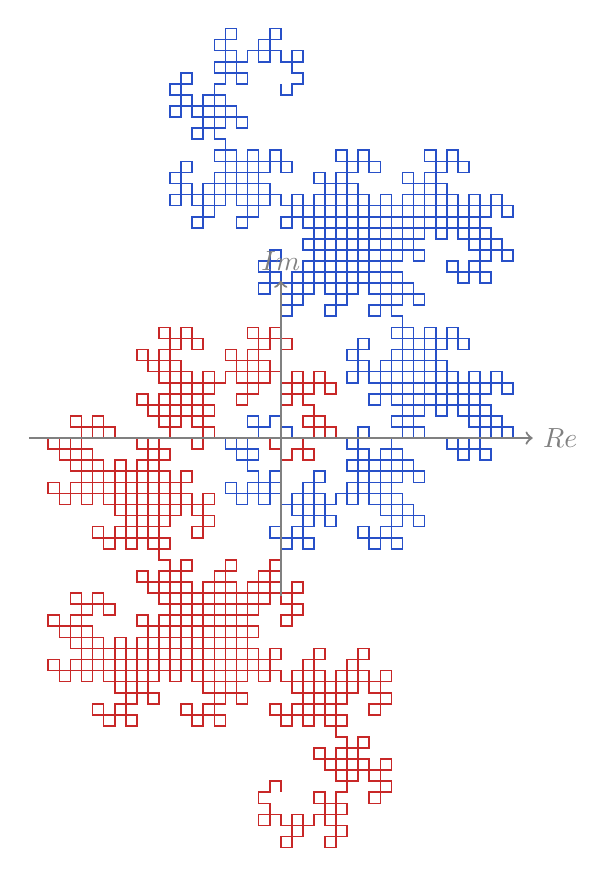
\begin{tikzpicture}[scale=0.8]
    
        \draw [draw=dragonBlue, line width=0.6pt]
        [l-system={Dragon, step=2.5pt, axiom=FX, order=10, angle=90}]
        lindenmayer system;
        
        \draw [draw=dragonRed, line width=0.6pt, rotate=180]
        [l-system={Dragon, step=2.5pt, axiom=FX, order=10, angle=90}]
        lindenmayer system;
        
        \draw[->, thick, gray] (-4,0) -- (4,0) node[right] {\lr{$Re$}};
        \draw[->, thick, gray] (0,-2.5) -- (0,2.5) node[above] {\lr{$Im$}};
    \end{tikzpicture}
    \caption{نمایش «اژدهای دوقلو»؛ دو منحنی که بدون همپوشانی در هم قفل شده‌اند.}
    \label{fig:twin_dragon}
\end{figure}

\section{نتیجه‌گیری}
منحنی اژدها ثابت می‌کند که قوانین بازگشتی ساده می‌توانند ساختارهای پیچیده‌ی ریاضی تولید کنند. ترکیب آن با نظریه اعداد، دریچه‌ای نوین به سوی فشرده‌سازی اطلاعات و رمزنگاری باز کرده است و پژوهش‌ها پیرامون توابع مختصاتی آن همچنان در سال ۲۰۲۵ ادامه دارد.

\section*{سپاس‌گزاری}
از استاد ارجمند، \textbf{جناب آقای دکتر محمود امین طوسی}، بابت تدریس مفاهیم بنیادین و راهنمایی‌های ارزشمند در درس مبانی کامپیوتر صمیمانه تشکر می‌نمایم.

\bibliographystyle{amsplain}

\begin{thebibliography}{5}
\begin{latin}

\bibitem{davis1970} 
C. Davis and D. Knuth, \textit{Number representations and dragon curves}, J. Recreational Mathematics, 3 (1970), 66--81.

\bibitem{knuth}
D. E. Knuth, \textit{Selected Papers on Fun \& Games}, CSLI Publications, 2011.

\bibitem{arxiv2025}
F. Wen and S. Akiyama, \textit{The coordinate functions of the Heighway dragon curve}, arXiv preprint arXiv:2506.05541 (2025).

\end{latin}
\end{thebibliography}

\end{document}